\section{Constructed illustrative walkthrough}
\label{sec:walkthrough}

The following example is an author-constructed illustration of the relationship between the Research Map and the inspected implementation. It concerns a fictional municipal library and a hypothetical collection of digitized historical photographs. No project was created in the application for this example; no model or Research Starter call was made, no participant supplied data, and no map was completed or exported. The formulations below are illustrative inputs, not responses produced by the agent. This distinction matters because the example can explain a possible authoring path but cannot demonstrate usability, effectiveness, or the quality of a completed research design.

\subsection{Initial synthetic plan}

Suppose that the researcher begins with the question: ``How can metadata standardization support the discovery of historical photographs in a fictional municipal library?'' A corresponding general objective is to analyze how metadata standardization could support discovery in that collection. Three specific objectives are constructed: (OE1) identify descriptive metadata fields; (OE2) examine search patterns in a fictional catalogue; and (OE3) propose guidance for describing and finding the photographs. Three objectives lie within the original map's suggested range of three to six \cite{franca2026map}; their selection here is illustrative, not an agent decision or an author appraisal of methodological adequacy.

The literature outline could contain metadata quality, subject access, and catalogue search. A development outline could contain description of the fictional collection, analysis of constructed search examples, and synthesis of guidance. These are labels for planning relations, not chapters written or sources retrieved. The inspected application represents links between topics and objectives and requires reference identifiers and justifications in its chapter workflow; because this example supplies no real bibliographic records, it is not presented as a set of entries that would pass those routes unchanged.

Table~\ref{tab:walkthrough-matrix} sketches the companion matrix. Every item is prospective. ``Expected output'' refers to an anticipated product of the proposed work, never to an observed result of a library study.

\begin{table}[htbp]
\centering
\small
\caption{Constructed objective--method matrix for the fictional library case. No records, searches, or outputs were collected or produced.}
\label{tab:walkthrough-matrix}
\begin{tabular}{>{\raggedright\arraybackslash}p{0.22\linewidth} >{\raggedright\arraybackslash}p{0.34\linewidth} >{\raggedright\arraybackslash}p{0.34\linewidth}}
\hline
Objective & Planned information and treatment & Expected output \\
\hline
OE1: metadata fields & Constructed catalogue records; compare field presence and consistency & Inventory of fields and candidate gaps \\
OE2: search patterns & Constructed catalogue queries; classify query paths and retrieval descriptions & Map of possible discovery paths \\
OE3: guidance & Planned synthesis of OE1/OE2 and literature still to be verified & Draft rules for description and discovery \\
\hline
\end{tabular}
\end{table}

The actual application additionally stores a methodological classification and a general-objective synthesis row. They are omitted from this compact example, which is intended to explain the relation between specific aims and prospective means, rather than simulate a valid route submission. Whether the proposed inputs or treatments are appropriate would require a disciplinary judgment by a researcher.

\subsection{One upstream change}

Now suppose that the researcher narrows the question to: ``How can standardizing subject and date metadata support the discovery of historical photographs in a fictional municipal library?'' The revision specifies two metadata dimensions that the original question left open. It is not, by itself, evidence that the new question is better. It creates a reason to reconsider whether the general objective, each specific objective, the literature and development topics, and the matrix still address the selected problem.

The implementation distinguishes saving this wording as a draft from confirming it as academic content. Only a confirmed change to the problem triggers the versioned workflow's dependency handling. Its type-level rule can mark the general objective, specific objectives, topics, methodology, title, and final map as stale while retaining their text and history. It does not traverse each trace link to determine which particular sentence is affected. The researcher must inspect those items and decide whether to edit or reaffirm them. Figure~\ref{fig:walkthrough-revision} displays this hypothetical revision and its code-inspected consequence; no such action was executed on the fictional project.

\begin{figure}[htbp]
\centering
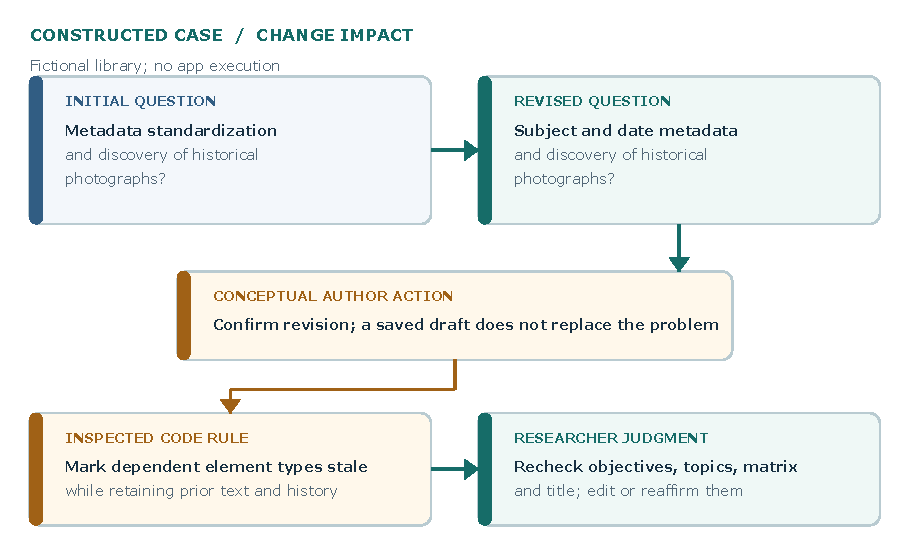
\includegraphics[width=\linewidth]{figures/walkthrough-revision.pdf}
\caption{Constructed change-impact illustration. The initial and revised questions are author-written examples. The stale-marking rule is based on inspected source code, but it was not run on this fictional project. The arrows do not represent observed user behavior or a generated response.}
\label{fig:walkthrough-revision}
\end{figure}

If the same example were entered in student authoring mode, submitting a validated stage would create a pending advisor review and an attempted e-mail notification, as described in Section~\ref{sec:system}. An authenticated advisor could approve the stage or request corrections; approval, rather than the e-mail, would permit the next transition. This conditional branch is included to explain the available workflow. No student submission, message delivery, advisor decision, or methodological rating occurred in this example. In advisor authoring mode, the external review request would not be required.

\subsection{What the illustration demonstrates}

The example makes two relations visible: the map decomposes a central question into objectives, topic structures, and prospective methods; and an upstream edit in the application calls for renewed human consideration of downstream content. The first relation comes from the method's planning documents \cite{franca2026map,franca2026detail}; the second is a behavior supported by inspection of the versioned workflow code, not by execution of this constructed case. The limited local wording checks previously performed on the example found no structural or lexical messages for the revised problem and objectives. They did not validate the topics, matrix, persistence route, coherence of the research design, or any participant outcome.

Final-map review would be advisory, and a PDF or DOCX would require an eligible workflow state and either current final approval or an explicitly labelled draft. No such report was generated for this example. Thus the walkthrough explains a traceable design and a possible revision path; it does not establish that the agent improves planning, that an e-mail was received, or that the hypothetical library project would yield its expected outputs.
